\chapter{Theoretical Background}
\label{chap:2_theoretical_background}
\textcolor{myred}{In the previous chapter, we have argued that multiple robotic tasks would benefit from exploiting the semantic information inferred from spatial and temporal organization of the environments that surrounds the robot. We have chosen the object search (OS) problem to explore this idea, which aims to estimate a target object's location in a large unknown environment, usually with a camera attached to a mobile robot. We believe investigating this problem can enlarge our understanding regarding the benefits of employing semantic information to expand the robot's perception. }

\textcolor{myred}{This chapter presents a theoretical background detailing techniques used throughout this thesis. The OS problem requires the robot to map the unknown environment and to estimate its position simultaneously. SLAM systems fulfill these requirements, as it computes the state estimation and builds an environment representation. Hence, we address the basic concepts of such systems and mobile robotics in general, from the individual localization and mapping problems to how they are combined into the SLAM systems. Besides, we cover the generic and central formulation of OS problems, which is the basis for the works presented in Chapters~\ref{chap:3_text_os_system} and~\ref{chap:4_temporal_os_system}.}

\section{Perception}
\label{sec:chap2_perception}

\subsection{Text Localization and Recognition}
\label{subsec:chap2_ocr}
Text can be embedded into documents or scenes as a means of communicating information, and it is considered one of the most expressive means of communications~\cite{Ye2014Text}. The process of Optical Character Recognition (OCR) aims to detect and recognize text in printed materials, images or videos, to then convert it into a digitized form so that machines can manipulate the digital text~\cite{Ye2014Text, Islam2017Survey}. The OCR process has been in the spotlight for several years~\cite{Islam2017Survey}. The motivation for such attention from the research community is that text provides meaningful information to be used in many applications. Besides, OCR is a complex problem due to the variety of languages, fonts, and styles in which text can be written, along with the complex rules of languages~\cite{Islam2017Survey}.

There are two methodologies commonly used in OCR systems, \textit{integrated} and \textit{stepwise}~\cite{Ye2014Text}. The integrated methodology recognizes words when the detection procedures share information with character classification and relies on joint optimization strategies, as shown in Fig.~\ref{chp02_fig:integrated_methodlogy}. On the other hand, stepwise methodology has separated detection and recognition modules. Besides, it uses a feed-forward pipeline to detect, segment, and recognize text regions, shown in Fig.~\ref{chp02_fig:stepwise_methodology}~\cite{Ye2014Text}. Lastly, it relies on a feedback procedure from text recognition to text detection to reduce false detections.

\begin{figure}[ht!]
    \footnotesize
    \centering
    \begin{subfigure}[b]{0.9\columnwidth} 
        \includegraphics[width=\textwidth]{figs/integrated_methodology.png} 
        \caption{Integrated  Methodology}    
        \label{chp02_fig:integrated_methodlogy}
    \end{subfigure}\\ 
    \begin{subfigure}[b]{0.9\columnwidth} 
        \includegraphics[width=\textwidth]{figs/stepwise_methodology.png} 
        \caption{Stepwise Methodology} 
        \label{chp02_fig:stepwise_methodology}
    \end{subfigure}~
    \caption[Frameworks of two popular text detection and recognition methodologies.]{Frameworks of two popular text detection and recognition methodologies, where (a) is the Stepwise methodology, and (b) is the Integrated methodology. Adapted from~\citet{Ye2014Text}.}
    \label{chp02_fig:problems_robotics}
\end{figure}  

The latter methodology usually employs a coarse-to-fine strategy, which is done in four steps: localization, verification, segmentation, and recognition~\cite{Ye2014Text}. The goal of the first step, localization, is to coarsely classify components and groups into candidate text regions. In the second step, verification, such regions are further classified into text or non-text regions. The third step, segmentation, separates the characters in a way that exclusive, accurate outlines of image blocks remain for the recognition step. Lastly, the recognition step converts image blocks into characters. It is also possible that some stepwise methodologies ignore the verification and/or segmentation steps. Further, another adaptation is the inclusion of additional steps to perform text enhancement and/or rectification~\cite{Ye2014Text}. 

One of the leading methods in scene text detection is based on detecting characters, such as the one proposed by ~\citet{Neumann2012Realtime}~\cite{Zhang2016Multi}. It is an end-to-end real-time scene text localization and recognition method based on the stepwise methodology~\cite{Neumann2012Realtime, Ye2014Text}. Neumann and Matas addressed the character detection problem as an efficient sequential selection from the set of Extremal Regions (ERs) to achieve real-time performance. Such ER is a character detector that analyses image regions whose outer boundary pixels have higher values than the region itself. It is robust to blur, illumination, colour, and texture variation. Additionally, it also handles low-contrast text~\cite{Neumann2012Realtime}. The pixels within each ER's bounding box are described by a class of region descriptors that serve as features for the character classification.

In a given grayscale image, Figure~\ref{chp02_fig:ocr_intensity_channel}, the authors do the text localization by estimating the probability of each ER being a character using a set of features, Figure~\ref{chp02_fig:ocr_ers_first_stage}. The verification step is done by selecting only the ERs from the previous step with locally maximal probability (of being a character), Figure~\ref{chp02_fig:ocr_ers_second_stage}. Since the verification step aims to eliminate not promising character candidates, the authors further classify the high-likely ERs with more computationally expensive features to improve the character classification. Then, they group the verified ERs into words and select the most probable character segmentation, Figure~\ref{chp02_fig:ocr_grouping}. The grouping is computed with a highly efficient exhaustive search with feedback loops. To get the text detected, Figure~\ref{chp02_fig:ocr_text_recognized}, the average run time of the proposed method on a $800 \times 600$ image is 0.3s on a standard PC~\cite{Neumann2012Realtime}. The method proposed by Neumann and Matas achieved state-of-the-art text localization results when evaluated in two public datasets. Besides, they were the first ones to report results for the end-to-end text recognition on the ICDAR 2011 Robust Reading competition dataset~\cite{Neumann2012Realtime}

\begin{figure}[ht!]
    \footnotesize
    \centering
    \begin{subfigure}[b]{0.25\columnwidth} 
        \includegraphics[width=\textwidth]{figs/source_image.png} \caption{} 
        \label{chp02_fig:ocr_source_image}        
    \end{subfigure}~
    \begin{subfigure}[b]{0.25\columnwidth} 
        \includegraphics[width=\textwidth]{figs/intensity_channel_extracted.png} \caption{} 
        \label{chp02_fig:ocr_intensity_channel}        
    \end{subfigure}~ 
    \begin{subfigure}[b]{0.25\columnwidth} 
        \includegraphics[width=\textwidth]{figs/ers_selected_first_stage.png} \caption{}
        \label{chp02_fig:ocr_ers_first_stage}        
    \end{subfigure}\\
    \begin{subfigure}[b]{0.25\columnwidth} 
        \includegraphics[width=\textwidth]{figs/ers_selected_second_stage.png} \caption{} 
        \label{chp02_fig:ocr_ers_second_stage}        
    \end{subfigure}~ 
    \begin{subfigure}[b]{0.25\columnwidth} 
        \includegraphics[width=\textwidth]{figs/text_lines_region_grouping.png} \caption{}
        \label{chp02_fig:ocr_grouping}        
    \end{subfigure}~ 
    \begin{subfigure}[b]{0.25\columnwidth} 
        \includegraphics[width=\textwidth]{figs/ers_text_lines_text_recognized.png} \caption{}
        \label{chp02_fig:ocr_text_recognized}        
    \end{subfigure}\\[0.1cm]
    \caption[Text localization and recognition overview.]{Text localization and recognition overview, in which (a) is the source image, (b) is the extracted intensity channel, (c) is the ERs selected by the first stage of the sequential classifier, (d) is the ERs selected by the second stage of the classifier, (e) is the text lines found by region grouping, and (f) is the only ERs in text lines selected and text recognized by an OCR module. Extracted from~\cite{Neumann2012Realtime}.}
    \label{chp02_fig:ocr_papger_overwall}
\end{figure}  

%They pose the character detection problem as a sequential selection from the set of Extremal Regions. Then, the recognition of candidate regions is done in a separete OCR stage using synthetic fonts~\cite{Almazan2014Word}

\subsection{You Only Look Once (YOLO)}

Generic object detection problem is defined as determining whether there are instances of objects from predefined categories in an given image. For the present instances, it is also necessary to return their spatial location and extent~\cite{Liu2020Deep}. This problem is also known as generic object category detection, object class detection, or even object category detection~\cite{Liu2020Deep}. It focuses on detecting a broad range of natural categories instead of specific object category detection, where only a narrower predefined category of interest may be present, such as faces, pedestrians, or cars. Nowadays, the research community is more interested in detecting highly structured objects, like cars, bicycles, and airplanes, and articulated objects, such as humans and pets, rather than unstructured scenes (e.g., sky, grass, and cloud)~\citep{Liu2020Deep}. Regarding the spatial location and extend of an object within an image, like the detected objects in Figure~\ref{chp02_fig:yolo_object_classification}, it can be defined coarsely using a bounding box~\cite{Everingham2010Pascal, Redmon2016You}, which is a rectangle tightly bounding the object, Figure~\ref{chp02_fig:yolo_object_detection}, a precise pixel-wise segmentation maks~\cite{Zhang2013Object}, Figure~\ref{chp02_fig:yolo_semantic_segmentation}, or a closed boundary~\cite{Russell2008Labelme, Lin2014Microsoft}, Figure~\ref{chp02_fig:yolo_object_instance_segmentation}~\cite{Liu2020Deep}.

\begin{figure}[htbp]
%    \footnotesize
    \centering
    \begin{subfigure}[t]{0.25\columnwidth} 
        \includegraphics[width=\textwidth]{figs/yolo_object_classification.png} 
        \caption{Object classification} 
        \label{chp02_fig:yolo_object_classification}        
    \end{subfigure}~
    \begin{subfigure}[t]{0.25\columnwidth} 
        \includegraphics[width=\textwidth]{figs/yolo_object_detection.png} 
        \caption{Generic object detection \\ (Bounding box)} 
        \label{chp02_fig:yolo_object_detection}        
    \end{subfigure}~ 
    \begin{subfigure}[t]{0.25\columnwidth} 
        \includegraphics[width=\textwidth]{figs/yolo_semantic_segmentation.png} 
        \caption{Semantic segmentation}
        \label{chp02_fig:yolo_semantic_segmentation}        
    \end{subfigure}~ 
    \begin{subfigure}[t]{0.25\columnwidth} 
        \includegraphics[width=\textwidth]{figs/yolo_object_instance_segmentation.png} 
        \caption{Object instance segmentation}
        \label{chp02_fig:yolo_object_instance_segmentation}        
    \end{subfigure}
    \caption[Recognition problems related to generic object detection.]{Recognition problems related to generic object detection. This figure shows (a) image level object classification, (b) bounding box level generic object detection, (c) pixel-wise semantic segmentation, and (d) instance level semantic segmentation. Extracted from~\cite{Liu2020Deep}.}
    \label{chp02_fig:object_detection.}
\end{figure} 

Recently, deep learning-based techniques have been proposed to deal with the object detection problem~\cite{Redmon2016You}. Deep learning has been used to solve many other challenging tasks, in areas such as image classification~\cite{Krizhevsky2012Imagenet, He2016Deep} and language modeling~\cite{Gong2018Frage, Dai2019Transformer}\cite{He2021Automl}. Deep learning techniques have arisen as powerful techniques for learning feature representations automatically from data~\cite{Liu2020Deep}. The success of deep learning in general in these areas is partly due to the rapidly developing computational resources, such as powerful graphical cards, the availability of big training data, and the effectiveness of deep learning to extract hidden representations from images, texts, and videos~\cite{Wu2020Comprehensive}.

A popular deep learning approach for object detection that has been improved since its first version is called YOLO~\cite{Redmon2016You}. The name is an acronym and is short for ``\textit{You Only Look Once}'', which partially explains the general idea of the approach. The YOLO's authors have entirely abandoned the initial object detection paradigm of ``\textit{proposal detection + verification}''. Instead, they followed an entirely different idea: to apply a single neural network to the whole image. This idea made YOLO the first one-stage object detector in the deep learning era (where the name comes from)~\cite{Zou2019Object}. Thanks to this unified approach, YOLO detects objects extremely fast, processing images in real-time at 45 frames per second (FPS)~\cite{Redmon2016You}. To compare, the best object detector before YOLO, called Faster RCNN, processes images at 5~7 FPS~\cite{Liu2020Deep}.

\citet{Redmon2016You} approached object detection as a regression problem, straight from image pixels to bounding box coordinates and class probabilities~\cite{Liu2020Deep}. Each image is evaluated once in their system by a single neural network that predicts bounding boxes and class probabilities. Due to this single network detection pipeline, YOLO can be optimized end-to-end directly on detection performance~\cite{Redmon2016You}.

YOLO divides an image into an $U \times U$ grid, and each grid cell predicts $B$ bounding boxes and confidence scores for those boxes. These confidence scores reflect how confident the model is that the box contains an object. In addition, the score also suggests how accurate YOLO thinks the box is what it predicts. In the second image of Figure~\ref{chp02_fig:yolo_system_model}, the score of the bounding boxes is represented by their thickness. The thicker the bounding box, the higher the confidence that there is an object in that location. Here is important to mention that at this point, YOLO does not know which objects there are in the image. It just knows whether exist any and their locations. To find out the object classes within the image, YOLO predicts $C$ conditional class probabilities for each grid cell. These probabilities are conditioned on the grid cell containing an object. It means that YOLO is predicting that if there is an object in a cell, that object is an instance of the class with the highest probability. YOLO only predicts a set of class probabilities per grid cell regardless of the number of bounding boxes $B$ for each grid cell. The third image of Figure~\ref{chp02_fig:yolo_system_model} illustrates this prediction. Finally, YOLO multiplies the conditional class probabilities and the individual bounding box confidence predictions at the test time, which results in the class-specific confidence scores for each box. Hence, these scores encode both the probability of that class appearing in the bounding box and how well the predicted box fits the object, represented by the fourth image of Figure~\ref{chp02_fig:yolo_system_model}. Through a non-max suppression process, YOLO discards low-value bounding boxes and duplicated detections, resulting then in the final detections, illustrated by the fifth image of Figure~\ref{chp02_fig:yolo_system_model}.

\begin{figure}[ht!]
    \footnotesize
    \centering
    \begin{subfigure}[b]{\columnwidth} 
        \includegraphics[width=\textwidth]{figs/yolo_system_model.png} %\caption{SLAM} 
    \end{subfigure}
    \caption[YOLO's model detection as a regression problem.]{YOLO's model detection as a regression problem. The input image is initially divided into an $U \times U$ grid, and for each grid cell YOLO predicts $B$ bounding boxes, confidence for those boxes, and $C$ class probabilities. Adapted from~\cite{Redmon2016You}.}
    \label{chp02_fig:yolo_system_model}
\end{figure}

Unlike sliding window and region proposal-based techniques, YOLO reasons globally about the image when making predictions, processing the entire image during training and test time~\cite{Redmon2016You}. Hence, it implicitly encodes contextual information about classes and their appearance. Besides, YOLO learns generalizable representations of objects. In one of its experiments, YOLO was trained on natural images and tested on artwork, outperforming top detection methods proposed by the research community~\cite{Redmon2016You}. However, despite its significant improvement in detection speed, YOLO suffers from a slight drop in localization accuracy compared with two-stage detectors, especially for some small objects~\cite{Zou2019Object}.


\section{Kernel Density Estimation in grid maps} 

The process of computing the probability density function $f$ of any data sample $X = \{\bs{x}_1, \bs{x}_2,\bs{x}_3, \cdots, \bs{x}_n\}$ is called density estimation~\cite{Devroye1999Hilbert, Maffei2017Translating, Bhattacharjee2021KAGO}. The kernel density estimatation (KDE), $\hat{f}_h(\bs{x})$, is a non-parametric estimate of $f$ computed at point $\bs{x}$, defined as
\begin{equation}
\hat{f}_h(\bs{x}) = \frac{1}{n}\sum^n_{i=1}K_h(\bs{x} - \bs{x}_i)
\label{chp02_eq:kde}
\end{equation}
where $K_h(d)$ is a circular kernel function that operates over all points at distance $d \leq h$ from $\bs{x}$, and $h$ is called the bandwidth of the kernel~\cite{Silverman1986Density, Jones1992Class}. 

For any given point $\bs{x}_i \in X$ where $1 \leq i \leq n$, the KDE on dataset $X$ is used to estimate the likelihood of a point $\bs{x}_i$ being drawn from $X$. The probability estimated through the kernel density estimator may be interpreted as the “point density” at any $\bs{x}_i \in X$~\cite{Devroye1999Hilbert, Bhattacharjee2021KAGO}.

A variety of kernel profiles may be applied for estimating the density using KDE. Even though the Gaussian kernel is one of the most frequently used kernel functions, other kernel profiles are used by the research community~\cite{Silverman1986Density, Maffei2015Fast}. Below we show the uniform, gaussian, and the inverted ones:
\begin{equation}
UK_{h}(d) = \left\{\begin{matrix}a & \text{, if}~d \leq r\\ 
0 & \text{~~, otherwise} \end{matrix}\right.
\end{equation}
\begin{equation}
GK_{h}(d) = \frac{1}{h\sqrt{2\pi}}\exp\Big(-\frac{1}{2}\frac{d^2}{h^2}\Big)
\end{equation}
\begin{equation}
IK_{h}(d) = \left\{\begin{matrix}
h(b+c) - (\sqrt{h^2 - d^2})c~&\text{, if}~d \leq h\\ 
0~~~~~~~~~~~~~~~~~~~~~~~~~~~~~&\text{~~, otherwise}
\end{matrix}\right.
\end{equation}
where $d$ signifies the distance from a kernel centre $\bs{x}$ to the target point $\bs{x}_i$, $r$ is the radius of the kernel, and $a$ is the height of the uniform kernel — typically $a = 1 / (\pi r^2)$. The kernel bandwidth $h$ is also known as the smoothing factor that controls the smoothness of the curve obtained from the KDE function. A higher value of $h$ ensures a smoother curve of the kernel~\cite{Bhattacharjee2021KAGO}. For $IK(\cdot)$, $b$ and $c$ are respectively the height of the uniform circular kernel and the length of the semi-axis of the oblate ellipsoid~\cite{Maffei2015Fast}. Figure~\ref{chp02_fig:kernel_profiles} shows these three kernel profiles in their 2D and 2${~}^1/_2$D shapes. 

\begin{figure}[htbp]
%    \footnotesize
    \centering
    \begin{subfigure}[t]{.5\columnwidth} 
        \includegraphics[width=\textwidth]{figs/kde_scale2.png} 
%        \caption{}
        \label{chp02_fig:kde_scale}        
    \end{subfigure}\\\vspace{-.4cm}    
    \begin{subfigure}[t]{0.25\columnwidth} 
        \includegraphics[width=\textwidth]{figs/kde_uk_2d.png} 
        \caption{2D Uniform kernel} 
        \label{chp02_fig:kde_uk_2d}        
    \end{subfigure}~
    \begin{subfigure}[t]{0.25\columnwidth} 
        \includegraphics[width=\textwidth]{figs/kde_gk_2d.png} 
        \caption{2D Gaussian kernel} 
        \label{chp02_fig:kde_gk_2d}        
    \end{subfigure}~ 
    \begin{subfigure}[t]{0.25\columnwidth} 
        \includegraphics[width=\textwidth]{figs/kde_ik_2d.png} 
        \caption{2D Inverted Kernel}
        \label{chp02_fig:kde_ik_2d}        
    \end{subfigure}\\ 
    \begin{subfigure}[t]{0.25\columnwidth} 
        \includegraphics[width=\textwidth]{figs/kde_uk_25d.png} 
        \caption{2${}^1/{}_2$D Uniform kernel} 
        \label{chp02_fig:kde_uk_25d}        
    \end{subfigure}~
    \begin{subfigure}[t]{0.25\columnwidth} 
        \includegraphics[width=\textwidth]{figs/kde_gk_25d.png} 
        \caption{2${}^1/{}_2$D Gaussian kernel} 
        \label{chp02_fig:kde_gk_25d}        
    \end{subfigure}~ 
    \begin{subfigure}[t]{0.25\columnwidth} 
        \includegraphics[width=\textwidth]{figs/kde_ik_25d.png} 
        \caption{2$1/2$D Inverted Kernel}
        \label{chp02_fig:kde_ik_25d}        
    \end{subfigure}  
    \caption[Different kernel profiles shown in 2D and 2$1/2$D.]{Different kernel profiles shown in 2D and 2$1/2$D. Adapted from~\cite{Maffei2017Translating}.}
    \label{chp02_fig:kernel_profiles}
\end{figure} 

The KDE is a fundamental tool in statistics~\cite{Devroye1985Nonparametric, Silverman1986Density, Devroye2001Combinatorial, Scott2015Multivariate} and machine learning~\cite{Scholkopf2002Learning, Gretton2012Kernel, Muandet2017Kernel}. However, it can also be used in many other fields, such as robotics, like in work proposed by~\citet{Maffei2015Fast}. The authors proposed an efficient KDE-based observation model for a localization approach in their work. The KDE is estimated considering the density of free space cells in a 2D grid map, as these cells are more abundant and less noisy than the obstacle cells. One big advantage of using KDE for robotic applications is that it is orientation independent and has a low computational cost~\cite{Maffei2015Fast}. Their KDE of free space surrounding a point $\bs{x}$ is computed through an equation similar to Equation~\ref{chp02_eq:kde}:
\begin{equation}
\hat{f}_h(\bs{x}) = \frac{1}{n}\sum^n_{i=1}s(\bs{x})K_h(\bs{x} - \bs{x}_i)
\label{chp02_eq:free_space_kde}
\end{equation}
where the function $s(\cdot)$ is defined as

\begin{equation}
s(x) = \left\{\begin{matrix}1 \text{, if}~\bs{x}~\text{is inside a free space cell}\\ 
              \hspace{-3.2cm} 0 \text{, otherwise.}\end{matrix}\right.
\end{equation}

Figure~\ref{chp02_fig:kde_uniform} shows the Equation~\ref{chp02_eq:free_space_kde} with an uniform kernel applied to a 2D grid map. Given four map cells in four different spots of the map (1, 2, 3, and 4) indicated in Figure~\ref{chp02_fig:kde_points}, the circular KDE would consider the red cells highlighted in Figure~\ref{chp02_fig:kde_uk_2d}. The function $s(\cdot)$ in Equation~\ref{chp02_eq:free_space_kde} makes the KDE to consider only the free cells, as shown by the greenish cells in Figure~\ref{chp02_fig:kde_free_cells}. The free space density estimation for each cell, estimated with KDE, is illustrated in Figure~\ref{chp02_fig:kde_info}. In this image, it is possible to see that the larger the number of free cells within the kernel area, e.g. spot number 3, the higher the density. Besides, this simple example also demonstrates that KDE is invariant to ratations. The KDE for spots 1 and 4 are equal, even though the area of free cells for each spot is in different orientations (horizontal and vertical). Point 3 has the highest KDE, which is explained by the highest number of free cells under the kernel's coverage among all the four kernels.  

\begin{figure}[h!]
%    \footnotesize
    \centering
    \begin{subfigure}[t]{0.45\columnwidth} 
        \includegraphics[width=\textwidth]{figs/kde_points.png} 
        \caption{} 
        \label{chp02_fig:kde_points}        
    \end{subfigure}~
    \begin{subfigure}[t]{0.45\columnwidth} 
        \includegraphics[width=\textwidth]{figs/kde_area.png} 
        \caption{} 
        \label{chp02_fig:kde_area}        
    \end{subfigure}\\
    \begin{subfigure}[t]{0.45\columnwidth} 
        \includegraphics[width=\textwidth]{figs/kde_free_cells.png} 
        \caption{}
        \label{chp02_fig:kde_free_cells}        
    \end{subfigure}~ 
    \begin{subfigure}[t]{0.45\columnwidth} 
        \includegraphics[width=\textwidth]{figs/kde_info.png} 
        \caption{}
        \label{chp02_fig:kde_info}        
    \end{subfigure}
    \caption[Computing kernel density estimates in four different positions of an image.]{Computing kernel density estimates in four different positions of a map. The gray cells represent the unknown region, whereas the white ones the free space. In (a) we have the four spots to compute the kernel density, in (b) the area of each kernel, in (c) the free cells within the area of the kernel, and in (d) the computed free space density.}
    \label{chp02_fig:kde_uniform}
\end{figure} 

The idea of estimating the free space density with the aid of KDE was later used by Maffei and colleagues in a second work,~\citet{Maffei2015Using}. This time, they were interested in using a robot to construct a topological map, to then localize itself using a laser range finder and odometry information. Their proposed algorithm used an observation model based on kernel density estimates, similarly to their previous work,~\citet{Maffei2015Fast}. The difference, however, is that this observation model separates the map into regions denominated words, classified based on the density of free space estimated with the KDE, number of observations, and segmentation orientation~\cite{Maffei2015Using}. The robustness of the free space density estimation in this second work motivated the authors to pursue a third work,~\citet{Maffei2016Long}. Now,~\citet{Maffei2016Long} proposed a long-term place recognition, which extends their strategy that represents environment regions using words based on spatial density information extracted from laser readings. The novelty is in building multi-level words to account for possible changes in the observations of a place generated by non-static objects. For example, when a robot is in front of a door and estimates the free space density, the final KDE value will differ whether the door is open. For long-term operations, this may happen, and even though the density value is different, the region is still the same. 

\section{The Basics of Mobile Robotics}
\label{sec:chap2_basic_mobile_robotics}
Mobile robots perform several tasks that require them to be aware of their positions in the environment and the position of obstacles to avoid collisions. In most realistic scenarios where robots are deployed, such information is not directly available. Hence, the robots have to estimate it with their sensors, which provide noisy data from the environment~\cite{Thrun2006Probabilistic}.

The state estimation in mobile robotics can be summarized in four variables: 
\begin{itemize}
	\item $\bs{x}_t$: robot's pose at time step $t$. It is composed by a three dimensional vector containing $(x, y, \theta)^T$, in which $x,y$  represent the position and $\theta$ the orientation. A sequence of robot's poses from time step $0$ to time step $t$ is defined as ${\bs{x}_{0:t}= \{ \bs{x}_0, \bs{x}_1, \cdots, \bs{x}_t\}}$.
	\item $\bs{m}_i$: object $i$'s position in the environment. A list of $N$ objects, with $1 \leq n \leq N$, in the environment along with their properties is given by the vector $\bs{m} = (\bs{m}_1, \bs{m}_2, \cdots, \bs{m}_N)^T$.
	\item $\bs{u}_t$: control data at instant $t$, and it corresponds to the change of state in the time interval $(t - 1;t]$. The sequence of control data that takes the robot from the initial position to $\bs{x}_t$ is denoted by ${\bs{u}_{1:t} = \{\bs{u}_1, \bs{u}_2, \cdots, \bs{u}_t\}}$.
	\item $\bs{z}^i_t$: the $i$-th measurement made by the robot at instant $t$. The vector of all of them acquired at the same instant $t$ is $\bs{z}_t = (\bs{z}^1_t, \bs{z}^2_t, \cdots, \bs{z}^K_t)^T$, whereas $\bs{z}_{1:t} = \{\bs{z}_1, \bs{z}_2, \cdots, \bs{z}_t\}$ expresses the history of all observations.	
\end{itemize}

After defining the four variables that are the basic foundation for state estimation in mobile robotics, it is worth to explain their role in different estimation problems.  The set of controls $\bs{u}_{1:t}$ and measurements $\bs{z}_{1:t}$ are always known since the robot's sensors provide them. Inertial measurement units and wheel encoders are examples of sensors that provide control data, whereas lidars, sonars, and cameras measure the environment. The other two variables, robot's pose, $\bs{x}_{0:t}$, and environmental map, $\bs{m}$, are not necessarily known. Depending on the estimation problem, it is necessary to estimate different variables, like the three examples depicted in Figure~\ref{chp02_fig:problems_robotics}. In \textit{Localization}, Figure~\ref{chp02_fig:problems_robotics_localization}, the map is known in advance, and hence, only the robot's pose is estimated. The opposite happens in \textit{Mapping}, Figure~\ref{chp02_fig:problems_robotics_mapping}, as the map is built based on the known robot's pose. Lastly, in \textit{SLAM}, Figure~\ref{chp02_fig:problems_robotics_slam}, which combines the two previous problems, none of them is given a priori, and therefore, both are estimated simultaneously. 

\begin{figure}[ht!]
    \footnotesize
    \centering
    \begin{subfigure}[b]{0.7\columnwidth} 
        \includegraphics[width=\textwidth]{figs/caption_example.pdf} %\caption{SLAM} 
    \end{subfigure}\\[0.1cm]
    \begin{subfigure}[b]{0.31\columnwidth} 
        \includegraphics[width=\textwidth]{figs/localization_example.pdf} \caption{Localization} 
        \label{chp02_fig:problems_robotics_localization}
    \end{subfigure}~ 
    \begin{subfigure}[b]{0.31\columnwidth} 
        \includegraphics[width=\textwidth]{figs/mapping_example.pdf} \caption{Mapping}
        \label{chp02_fig:problems_robotics_mapping}
    \end{subfigure}~
    \begin{subfigure}[b]{0.31\columnwidth} 
        \includegraphics[width=\textwidth]{figs/slam_example.pdf} \caption{SLAM} 
        \label{chp02_fig:problems_robotics_slam}
    \end{subfigure}\\[0.1cm]
    \caption[Fundamental problems in mobile robots and their state estimation.]{Fundamental problems in mobile robots and their state estimation. It is estimated: (a) robot's pose, (b) map, (c) both of them simultaneously. Extracted from~\cite{Maffei2017Translating}.}
    \label{chp02_fig:problems_robotics}
\end{figure}  

Localization is the most basic perceptual problem in robotics. It aims to determine the robot's pose relative to a given map of the environment. Localization can also be seen as a problem of coordinate transformation, in which it is established a correspondence between the map coordinate system and the robot's local coordinate system~\cite{Thrun2006Probabilistic}.  There are multiple localization problems, and they are not equal in terms of their difficulty level. One characteristic that divides this problem into local and global localization is the awareness of the robot's initial pose. The former assumes that the initial robot's pose is known. Therefore, the problem becomes a sort of position tracking in which the noise in the measurements is adjusted in robot motion, commonly by a Gaussian distribution. On the other hand, the latter is unaware of the initial pose, making it perform the localization globally (where the name comes from) in the map. The global localization has a higher difficulty level than the local one, and one of its variations is even more challenging, the kidnapped robot problem. It addresses the problem of a localized robot being teleported to some other location in that the robot might believe it knows where it is while it does not.  Although a robot is rarely kidnapped in practice, recovering from localization failures is essential for autonomous robots. 

The formulation of the global localization problem is presented in Figure~\ref{chp02_fig:state_estimations}, which depicts a few iterations of the robot's pose estimation and how the variables are used. The map $\bs{m}$ is already known, whereas the $\bs{x}_{0:t}$ must be estimated based on the controls $\bs{u}_{1:t}$ and the measurements $\bs{z}_{1:t}$. For the case of local localization, the $\bs{x}_0$ is known and hence, it does not need to be estimated. Markov localization is a probabilistic algorithm that addresses all the localization problems mentioned earlier. It applies the Bayes filter, $p(\bs{x}_t \mid \bs{u}_{1:t}, \bs{z}_{1:t}, \bs{m})$, to transform a probabilistic belief at time $t-1$ into a belief at time $t$.

\begin{figure}[ht!]
    \footnotesize
    \centering
    \begin{subfigure}[b]{\columnwidth} 
        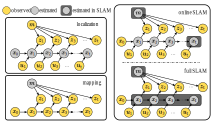
\includegraphics[width=\textwidth]{figs/graphical_models_loc_map_slam.pdf} %\caption{SLAM} 
    \end{subfigure}
    \caption[Graphical model of the fundamental mobile robotics problems.]{Graphical model of the fundamental mobile robotics problems: localization, mapping, and two SLAM variations. Adapted from~\cite{Maffei2017Translating}.}
    \label{chp02_fig:state_estimations}
\end{figure} 

Many other localization algorithms implement Markov localization in mobile robotics. Three of them have been in the spotlight for a long time and are prevalent in this field: Kalman filter, grid-based filter, and particle filter. The former filters predicts in linear dynamics and measurement functions~\cite{Leonard1991Mobile}, whereas the grid-based filter approximates the estimations by decomposing the state space into finitely many regions of the grid map~\cite{Burgard1998Integrating}. The key idea of the latter, particle filter, is to represent the estimation by a set of random state samples, called particles, drawn from the previous estimation. It can represent a much broader space of distribution, in contrast to the Kalman filter that is more strict to Gaussians~\cite{Dellaert1999Monte}. The particle filter implementation for mobile robotics is also known as Monte Carlo Localization (MCL), widely used in many different robotics applications for multiple robot types~\cite{Dellaert1999Monte, Thrun2006Probabilistic}. 

Mapping, for the case of the robot's poses are known, is the problem of generating consistent maps from noisy and imprecise measurement data~\cite{Thrun2006Probabilistic}. The estimated belief of the map, $p(\bs{m} \mid \bs{x}_{1:t}, \bs{z}_{1:t})$, considers the set of all measurements up to time $t$, $\bs{z}_{1:t}$, along with the robot's path defined by its history of all poses, $\bs{x}_{1:t}$, as shown in Figure~\ref{chp02_fig:state_estimations}. Comparing the graphical models of the localization and mapping problems in Figure~\ref{chp02_fig:state_estimations}, one can say that they are opposite in terms of which variable each estimates. This thought makes sense, since whereas the former relies on $\bs{m}$ to estimate $\bs{x}_{0:t}$, the latter relies on $\bs{x}_{0:t}$ to estimate $\bs{m}$. It is important to mention that the controls $\bs{u}_{1:t}$ play no role in this context, as the path is already known. Besides, the robot's initial pose $\bs{x}_0$ is omitted from the map estimation because no measures are taken when the robot is at that pose.

Similar to the localization problem that groups multiple localization types, the mapping problem also represents a general idea implemented by different map types. The feature-based maps represent the cartesian location of features, which are distinct objects in the physical world, extracted from the measurements, such as images from visual sensors or a vector of distances from a 2D lidar~\cite{Salas2013Slam++, Engel2014Lsd, Mur2015Orb}. The advantage of such a map type is the reduction of computational complexity, as the feature space has a lower dimension than the raw measurement. For example, the eight 3D edges of a boudingbox encircling a car are computationally cheaper to process than a point cloud from a 3D lidar. Another map type within the mapping problem is called location-based. It represents in each map component $\bs{m}_i$ the regions from the environment, regardless of whether they contain objects. This way, any location in the world has a label on the map, not only features. Occupancy grid maps are often considered the most popular location-based map~\cite{Thrun2006Probabilistic}. They discretize the environment into small portions called grid cells, which store information about the area it covers. In general, this information in each cell is a single value representing the probability that an obstacle occupies this cell. The size of the cells defines the map resolution, which brings a tradeoff between the level of details and the demand for memory resources. 

Lastly, Simultaneous localization and mapping (SLAM), also known as Concurrent Mapping and Localization, is undoubtedly the most fundamental and challenging problem in robotics~\cite{Thrun2006Probabilistic}. SLAM problems appear in scenarios where the environmental map is unavailable and the robot is unaware of its pose. In contrast to the other two problems presented earlier, which have to estimate either the map $\bs{m}$ or $\bs{x}_{1:t}$, in SLAM problems, the robot has to perform the estimation of both variables at the same time, as shown in Figure~\ref{chp02_fig:state_estimations}. Since the robot does not know its pose and there is no map, the pose $\bs{x}_0$ is assumed, by convention, to be $(0,0,0)^T$. The high difficulty level of SLAM comes from the double dependency of localization and mapping: to estimate the pose, the robot needs a map from the environment, whereas to estimate the map, the robot need to know its pose. 

The SLAM problem is divided into two forms based on what is estimated: online and full SLAMs. The former focus on estimating only the posterior over the current robot's pose $\bs{x}_t$ and the map $\bs{m}$, $p(\bs{x}_t, \bs{m} \mid \bs{z}_{1:t}, \bs{u}_{1:t})$. The full SLAM computes the same estimation, but with the entire robot's trajectory $\bs{x}_{1:t}$ along with the map $\bs{m}$, $p(\bs{x}_{1:t}, \bs{m} \mid \bs{z}_{1:t}, \bs{u}_{1:t})$.

The majority of the algorithms for the online SLAM problem are incremental, i.e., the idea is to estimate the posterior probability on the current robot state and map as the robot moves, discarding past measurements and controls once they have been processed. The Kalman and particle filters are also used in this context, besides the localization one as previously discussed. The Extended Kalman Filter is the basis of one of the earliest online SLAM approaches, linearizing motion and observation models, which usually are nonlinear, to perform the online SLAM estimations~\cite{Maffei2017Translating}. An online SLAM problem that is based on particle filter is known as Rao-Blackwellized particle filter (RBPF)~\cite{Murphy1999Bayesian, Doucet2000Rao, Grisettiyz2005Improving, Grisetti2007Improved}. In RBPF, each particle carries an individual grid map of the environment, representing a hypothesis of the robot's trajectory.  The number of particles is directly related to the map quality since the higher this number, the broader is the hypotheses variety. However, there is a cost associated with each particle, and hence,   it is not practical to increase the number of particles until the estimated map matches the physical world. 

The algorithms for the full SLAM problem calculate a posterior over the entire path, which solves an issue in the online SLAM problem. Discarding the previous states after estimating the current one, also known as Markov assumption, implies that the possible poor estimations in the past are not adjustable. In contrast, the full SLAM problems backpropagate to the previous estimations the error reduction computed in the current state calculation. GraphSLAM captures the essence of the full SLAM problem, since it calculates a solution for the offline problem over $\bs{x}_{1:t}$ and $\bs{z}_{1:t}$ in $\bs{m}$. Despite the advantage of improving previous state estimations, full SLAM algorithms are computationally heavy due to the optimization of nonlinear quadratic constraints. 

Explaining the fundamental problems of mobile robotics, from the simplest localization to the more complex SLAM problems, helps to understand why the OS works for unknown environments depend on a SLAM system. Since our works presented in the following chapters are designed for similar conditions (large and unknown environments), we opted to rely on GMapping~\cite{Grisetti2007Improved}. It is an online SLAM algorithm based on RBPF that provides a 2D grid map, and each cell contains a value that means whether the region it represents is unknown (to the SLAM system), occupied (obstacle), or free.

\section{The Boundary Value Problem (BVP) to deal with robotic problems}
Exploration is one of the robotic problems that the research community has been working on for many decades~\cite{Thrun2006Probabilistic}. Approaches that deal with this problem come in handy when a robot is deployed in an environment where a map is unavailable. This scenario requires the robot to safely move around within the environment at the same time that it builds the map. This problem has two fundamental requirements: the safety of the robot while it is moving and the preference for movements towards unexplored regions of the environment~\cite{Jorge2017Enabling}. A simple strategy to fulfil the safety requirement is to make the boundaries of obstacles to repel the robot. Similarly, the other requirement could be met by making the boundaries (frontiers) of unexplored regions attract the robot, as shown in Figure~\ref{chp02_fig:frontier_exploration}~\cite{Thrun2006Probabilistic}. Exploration approaches that are guided by the frontier of unexplored regions of the environment are commonly called frontier-guided~\cite{Jorge2017Enabling}.

\begin{figure}[ht!]
    \footnotesize
    \centering
    \begin{subfigure}[b]{\columnwidth} 
        \includegraphics[width=\textwidth]{figs/frountier_exploration.png} %\caption{SLAM} 
    \end{subfigure}
    \caption[Example of the two fundamental requirements of exploration at the boundaries of a partial map.]{Example of the two fundamental requirements of exploration at the boundaries of a partial map. The border of obstacles (black cells) has red arrows that represent the force that repels the robot. The border of unknown region (green cells) has green arrows that represent the force that attracts the robot. One way to update the potential field in the free space (white cells) is to consider a BVP, solving the Laplace equation considering the boundary-values in the green frontiers. Adapted from~\cite{Jorge2017Enabling}.}
    \label{chp02_fig:frontier_exploration}
\end{figure} 

Among the frontier-guided exploration approaches for exploratory tasks, we highlight the sequence of works proposed by Prestes and colleagues~\cite{Prestes2002Exploration, Prestes2003BVPExploration, Prestes2011Exploration}. Initially,~\citet{Prestes2002Exploration} proposed the use of a numeric solution to a boundary value problem (BVP) for the exploration problem. Their BVP exploration approach uses the gradient descent of the potential field generated over a grid to perform the map coverage with the robot. This potential field is computed with the finite difference method, by solving the Laplace equation,
\begin{equation}
\nabla^2 p(\bs{x}) = \sum^n_{i=1}\frac{\partial^2p(\bs{x})}{\partial x^2_i} = 0,
\label{chp02_eq:laplace_equation}
\end{equation} 
where $p(\bs{x})$ is the potential value at position $\bs{x}$ in the free space. In the grid map, the boundary of obstacles and unknown regions are considered Dirichlet boundary conditions. The potential value associated to unknown cells is the minimum, i.e. 0, whereas the same value associated to obstacle cells is the maximum, i.e. 1. The free cells have their potential value updated with Equation~\ref{chp02_eq:laplace_equation}~\cite{Prestes2002Exploration, Prestes2003BVPExploration}. However, as they are working with a discrete regular grid map, they used the Gauss-Seidel method for the numerical approximation of Equation~\ref{chp02_eq:laplace_equation}. Therefore, to update the potential value of free cells, they did
\begin{equation}
p(\bs{x}) = \frac{1}{4}(p(\bs{x}_l) + p(\bs{x}_r) + p(\bs{x}_u) +p(\bs{x}_b))
\label{chp02_eq:gauss_seidel}
\end{equation}
where $p(\bs{x}_l)$, $p(\bs{x}_r)$, $p(\bs{x}_u)$, and $p(\bs{x}_b)$ are the left, right, top and bottom cells neighboring the center and reference cell $p(\bs{x})$. Figure~\ref{chp02_fig:grid_potential} illustrates an example of these cells. 
\begin{figure}[ht!]
    \footnotesize
    \centering

	\includegraphics[width=.15\textwidth]{figs/grid_potential.png} %\caption{SLAM} 

    \caption[Representation of part of a 2D grid map $\bs{m}$.]{Representation of part of a 2D grid map $\bs{m}$. The potential field computed in relation to a cell centered at $\bs{x}$, considers the four neighbors cells on its left, right, bottom and up, $\bs{x}_l$, $\bs{x}_r$, $\bs{x}_b$, and $\bs{x}_u$, respectively.}
    \label{chp02_fig:grid_potential}
\end{figure} 

%potential field = solution of the laplace equation (which is an harmonic function)
The Equation~\ref{chp02_eq:gauss_seidel} applied to a 2D grid map to update the potential results in the exploratory behavior illustrated by Figure~\ref{chp02_fig:bvp_exploration}. The robot starts moving and it goes to the nearest frontier, Figure~\ref{chp02_fig:bvp_exploration_1}. Then it goes inside a room and maps it, Figures~\ref{chp02_fig:bvp_exploration_2} and~\ref{chp02_fig:bvp_exploration_3}. As there is no frontier within the room, the potential field guides the robot towards other frontiers to keep exploring, as shown in Figure~\ref{chp02_fig:bvp_exploration_4}. The BVP exploration approach uses the gradient descent of the potential field over a grid map to perform the map coverage.  
The angle of the robot's heading is computed based on the robot's current position on the potential field, i.e.
\begin{equation}
\theta = \arctan(p(\bs{x}_l) - p(\bs{x}_r), p(\bs{x}_u) - p(\bs{x}_b))
\end{equation}
where $\arctan(x,y)$ is the inverse tangent taken in the interval $[-\pi, \pi]$. The robot's speed can also be adjusted based on the potential field. The difference between the robot's orientation and the negative potential gradient direction $\theta$ for the current position represents how much the robot has to turn. Hence, this difference can be correlated to the robot's speed, i.e., the larger the difference, the slower is the robot's speed~\cite{Prestes2003BVPExploration}. Therefore, the BVP exploration has many advantages, including but not limited to smooth movements of the robot, easy understanding and implementation, and there are no local minima in the resulting potential field~\cite{Maffei2014Integrated, Jorge2015Ouroboros}.

\begin{figure*}[h!]
%    \footnotesize
    \centering

%    \begin{subfigure}[t]{0.2\columnwidth} 
	\hspace{-1cm}
        \includegraphics[width=.45\textwidth]{figs/bvp_exploration_map.png} 
        \label{chp02_fig:bvp_exploration_map}        
%    \end{subfigure}
\medskip
    \begin{subfigure}[t]{0.2\columnwidth} 
		\vspace{-5.5cm}
        \includegraphics[width=.75\textwidth]{figs/bvp_exploration_1.png} 
        \caption{} 
        \label{chp02_fig:bvp_exploration_1}        
    \end{subfigure}
    \begin{subfigure}[t]{0.2\columnwidth} 
		\vspace{-5.5cm}    
        \includegraphics[width=.75\textwidth]{figs/bvp_exploration_2.png} 
        \caption{}
        \label{chp02_fig:bvp_exploration_2}        
    \end{subfigure}\\~~~~~~~~~~~~~~~~~~~~~~~~~~~~~~~~~~~~~~~~~~~~~~~~~~~~~~~~~~~
    \begin{subfigure}[t]{0.2\columnwidth} 
		\vspace{-3.4cm}    
        \includegraphics[width=.75\textwidth]{figs/bvp_exploration_3.png} 
        \caption{}
        \label{chp02_fig:bvp_exploration_3}        
    \end{subfigure} 
    \begin{subfigure}[t]{0.2\columnwidth} 
		\vspace{-3.4cm}    
        \includegraphics[width=.75\textwidth]{figs/bvp_exploration_4.png} 
        \caption{}
        \label{chp02_fig:bvp_exploration_4}        
    \end{subfigure}    
    \caption[Exploration process with the potential field.]{Exploration process with the potential field. The trajectory followed by the robot is illustrated in the map, and four snapshots of the potential field during the exploration are shown in (a)-(d). Extracted from~\cite{Prestes2002Exploration}.}
    \label{chp02_fig:bvp_exploration}
\end{figure*} 



\section{Object search problem formulation}
The OS problem relies on an efficient strategy for finding a target object in a large unknown indoor environment. Since our works presented in this thesis are based on a 2D grid map, the search strategies from these works reason over the map $\bs{m}$. They estimate what cell $c$ is currently more promising to find the target object while minimizing the total search cost. We define cost as the distance traveled by the robot during the search, as the longer the robot's path, the higher is the amount of resources (battery and time) it spends. The robots we use throughout our experiments are equipped with a 2D lidar, to build a 2D grid map, RGB cameras, to gather visual cues for semantic information estimation, and RGB-D cameras to estimate the position of objects in relation to the robot's pose. All sensors are fixed to the robot's body, and hence, we consider only the movements performed by a ground mobile robot.  

Additionally, let $\varphi(c)$ be the probability distribution for a map cell, $c$, where the target object is in $\bs{m}$. Depending on the level of a priori knowledge of $\bs{m}$ and $\varphi(c)$, it is possible to address the OS problem in three different ways: 
\begin{itemize}
	\item $\bs{m}$ \textbf{and} $\varphi(c)$ \textbf{are known}: the problem becomes a sensor placement,  aiming to reduce the search cost by moving the robot straight to the cell $c$.
	\item \textbf{only} $\bs{m}$ \textbf{is known}: in case the map is available a priori (or acquired through a separate mapping step), the mobile robot should either rely on a generic probability distribution or move through the environment to gather information. The inspection performed by the robot is to get information about the objects and update the probability distribution. 
	\item $\bs{m}$ \textbf{and} $\varphi(c)$ \textbf{are unknown}: the robot needs to map the environment with the aid of a SLAM system, at the same time that it collects information to compute the probability distribution. Since the robot performs OS in an unknown environment, it has to tradeoff between expanding the mapped area and executing sensing actions to search for the target object carefully. This scenario is also known as the exploration vs. exploitation problem. 
\end{itemize}

In this thesis, the last two points are addressed in different works, Chapters~\ref{chap:3_text_os_system} and~\ref{chap:4_temporal_os_system}. In general, each of these works has an organisational semantic search strategy, i.e., it incorporates semantic information into the estimations to improve the performance. However, it is important to mention that these semantic search strategies consider common-sense knowledge, which is not environment-specific, and integrate high-level human concepts. In the context of this thesis, common-sense knowledge encodes semantic information inferred from characters signs and changes in the position of objects over time. Such information is valuable for our works because it reduces the search space and improves the search for a human-like performance.